% Latex Project Proposal
% SENG 474

\documentclass[journal]{IEEEtran}
\usepackage{graphicx}
\graphicspath{ {images/} }
\usepackage{array}
%-------------------------------------------------------------------------------------------------------------------

\begin{document}

\title{Final Report:\\\emph{Music Genre Classification Based on Song Lyrics}}

\author{Anna~Sollazzo,
        Henry~Hart,
        Jordan~Jay,
        Juan~Carlos~Gallegos,
        And~Robert~Craig \\ April 9th, 2018}

\maketitle

%-------------------------------------------------------------------------------------------------------------------

\begin{abstract}

    Our group aimed to explore the relationship between the lyrical content of a song and its associated music genre. Specifically, we had to construct different classification models to predict the genre of a song based solely on its lyrics. Our processes investigated the relationships between both a song's linguistic structure and its genre, as well as the lyrical content and genre. The dataset we used to train our model contained a set of 380,000 songs lyrics with their associated genre's. We implemented both a traditional classifier trained on a set of natural language (NL) features derived from the lyrics, as well as a deep learning model. After the classifiers were implemented, we then compared and contrasted their respective accuracies and errors.\par

\end{abstract}

%-------------------------------------------------------------------------------------------------------------------
\section{Introduction}

\IEEEPARstart{T}{H}{E} ability to correctly identify the genre of a particular song is crucial to allowing audiences to find related songs and is an important component to spreading music to masses of people. For example, without accurate genre classification, radio stations would not be able to specialize in the material they broadcast, and musicians may have difficulty producing consistent work. Having accurate and consistent genre classification alleviates some of these problems so musicians, marketers, and radio stations can produce coherent work and connect with people interested in their work. 
\par In order to perform the music genre classification that defines the relationships between the lyrical content of songs and their respective genres, our models had to be trained and tested on a large song lyric dataset. For this, we found a dataset that contained 380,000 song lyrics from Kaggle.com that was originally scraped from metrolyrics.com and is comprised of entities that include the song title, year, artist, genre, and lyrics \cite{KaggleDataset}. The classifications spanned 10 genres: country, electronic, folk, hip-hop, indie, jazz, metal, pop, R\&B, and rock. Before training our models on this data, we preprocessed the entire dataset by cleaning it (e.g. removing the relatively few songs without given genres) and ensuring the consistency of lyrical notation through systematic replacement of lyrical annotation (e.g [Chorus] is replaced with the text of the chorus). After which, we parsed our cleaned dataset into a feature set containing parts of speech (POS), frequency, word count, syllable count, and rhyme scheme. This feature set was essential to training our Support Vector Machine and was generated using NL techniques and tools such as Python Natural Language Tool Kit \cite{NLTK}. However, to train our neural net we only required raw and unstructured lyric data therefore no parsing was required for it. To ensure the quality and accuracy of the our final SVM and neural net models, we had to breakdown our data into the following test set of 80\% of our data for training, and 20\% for testing. Once both of our models were completed, we evaluated their classification precision and accuracy. Furthermore, we analyzed the dispersal of model errors over classes to check our intuition regarding both models to understand their areas of confusion. For example, whether the models frequently misclassify a song of a particular genre as another. \par


%-------------------------------------------------------------------------------------------------------------------

\section{Related Work}

There existed numerous attempts at classifying songs into genres solely by their lyrical content using neural networks and more traditional models such as SVM, k-nearest neighbor, etc.
Tsaptsinos \cite{tsaptsinos} extended the use of hierarchical attention networks (HAN) -- a type of recurrent neural network previously proposed and employed by Yang et al. \cite{Yang} for document classification -- to the lyrics-based music genre classification problem, demonstrating the model's ability to outperform the Long Short-Term Memory (LSTM) model when classifying across 117 genres. The HAN model performed particularly well when attention was placed at the line-level, as opposed to the segment level; that is, the model's accuracy benefited from considering lines individually instead of a block of lines (e.g. a refrain) as a whole unit. \par

More traditional models such as SVM, k- nearest neighbor, and random forests have found comparable success in lyrics-based genre classification. However, these models required preprocessing of the lyrics using NLP techniques to generate lyric feature sets for training. Canicatti \cite{canicatti} used song metadata (length and beats per minute), as well as word frequency vectors derived after stop word removal and word stemming, to train four models to classify five genres. Random forests outperformed the others, with a top accuracy of 47.35 percent. \par

Similarly, Mayer et al. \cite{mayer} trained several classifiers on basic features (e.g word count, line count) as well as more complex statistics such as POS tag frequency, occurrences of simple rhyme schemes (e.g. AABB, ABAB, ABBA and AA), and the proportion of unique terms used in rhyming. Their SVM that was trained on word count, line count, POS data, and rhyme data performed best, with an accuracy of 33.47 percent over ten genres. The team concluded that, in all cases, the inclusion of derived features in training data outperformed the traditional bag of words approach. Notably, both Canicatti and Mayer et al. suggested that a portion of their error may have come from their choice to remove lyrical annotation denoting repetition (e.g. "[chorus]" or "(x2)" ) instead of expanding them with the appriopriate sections (e.g. lyrics of chorus). \par

%-------------------------------------------------------------------------------------------------------------------
\section{Project Implementation}
The following subsections detail the implementation of the four major project components. 

\section{Data Cleaning}

Our first essential task was to clean the data in order to eliminate non-viable training examples and unecessary fields. After being run through the cleaner, all elements contained only the song name, genre classification, and lyrics. Any entry with a 'non-available' genre, lyrics that were too short for analysis (an arbitrary boundary of fewer than five lines), non english text, or nonsensical text (eg. all punctuation) were also removed. Additionally, the cleaner used regular expressions to systematically locate lyrical notation denoting repetition, i.e. (x2), and replaced it with the relevant text. This partially eliminated a source of error that was identified by Canicatti and Mayer et al. However, due to formatting inconsistencies we were not able to replace the notation for a song's chorus with the text itself. Instead, we used the count of these annotations in the NL feature set for the SVM and included them in the vocabulary for the neural network. Upon successfully cleaning the dataset it was reduced from 380,000 to 175,000 song entries.

\begin{figure}[h]
\centering
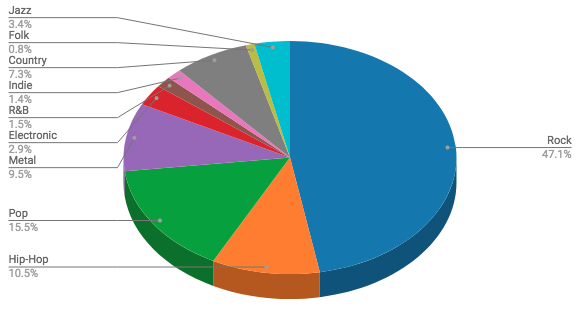
\includegraphics[width=9cm]{Figure_1}
\caption{Distribution of genre's across the dataset.}
\end{figure}

\section{NL Feature Set Generation}

Among the data preprocessing, the generation of a NL feature set for use by the SVM was also required. The NL feature set generated for each song has 22 features which were extracted using Python NLTK (See Table I). These features fall broadly into three categories: text aggregations, part of speech (POS) counts, and rhyme scheme analysis. The text aggregations included features such as average number of syllables per line and word count, while aimed to help the model learn the general shape of the lyrics. The POS counts recorded the semantic breakdown of the lyrics, though infrequently used POS were not included in the feature set. While the categorizations provided by NLTK are extremely fine grained, in an effort not to overwhelm our model with features we chose to bucket them into broader categories. For example, comparative adjectives and superlative adjectives were both classed as simply adjectives which may have resulted in some loss of accuracy. Finally, we used the Carnegie Mellon Pronunciation dictionary to perform rhyme scheme analysis. Due to the differences between the vocabularies of our lyrics and dictionary we were unable to access the phonetic breakdown of certain words. However, in general we were able to generate a rhyme scheme string for each set of lyrics and were encoded using letters. We contemplated using these raw encodings but observed that the model might not recognize the similarity between songs without identical rhyme schemes. Therefore, we opted instead to include counts of three common rhyme scheme sequences - aa, abba, abab, in the feature set.

\begin{table}[h!]
    \label{tab:table1}
    \centering
    \caption{Complete Feature Set}
    \begin{tabular}{ll}
       & \\
      \hline
      
	1. Annotation Count & 12. Adjective Count \\
	2. Syllables Per Line & 13. Verb Count \\
	3. Total Syllable Count & 14. Noun Count \\
	4. Pre-Determiner Count& 15. Preposition Count \\
	5. Determiner Count & 16. Pronoun Count \\
	6. Possessive Ending Count & 17. Conjunction Count\\
	7. Cardinal Digit Count & 18. Adverb Count\\
	8. Particle Count & 19. Existential There Count \\
	9. Interjection Count & 20. AA Rhyme Scheme Count \\
	10. Modal Count (i.e. Could, Will)  & 21. ABAB Rhyme Scheme Count \\
	11. Most Frequent Word Count & 22. ABBA Rhyme Scheme Count
	
    \end{tabular}
\end{table}

\section{SVM}

After cleaning our lyrics and extracting the necessary NL features to be used as a feature set for training our models, we used the SVM classifier available from Scikit-Learn. We experimented with some of the hyperparameters that were available within the Scikit-Learn library, in particular the different kernel functions and slack coefficients to find the optimal parameters for training our models.

For training and testing our models, we used a 80\% train and 20\% test split, and ran the model with the Linear, Poly, Sigmoid, and RBF kernel functions. For each kernel function, we tried slack variable coefficients 1, 50, and 100. The early results showed that Sigmoid performed consistently worse in terms of accuracy than the other functions therefore, due to time and computational constraints, we stopped training it early on in the process.

	In total, we trained SVMs on three different datasets. The first, separated the dataset into either being Rock or not Rock, before training our models. The second, performed multi-class classification on our entire dataset. Finally, our third dataset, was a stratified dataset that contained an equal distribution of each of the ten genres.
	
	Our initial goal for creating the Rock or not Rock SVM was to test the features that we had extracted from the dataset before transferring those same features to multi-class classification. The model that we trained had an accuracy of 65\% on the features that we extracted from the lyrical data, in comparison a random classifier that always chose not Rock had an accuracy of 53\%. We then used those same features on both the non-stratified and stratified datasets to both determine how the overabundance of Rock songs found in the dataset influenced the models that we trained, and how well each of our models performed on the ten genres. Furthermore, the model trained on the stratified dataset could then be compared with results found in related works along with our Recurrent Neural Network.  


\section{RNN}

TODO::

\section{Results}

The following subsections detail the results from our SVM and RNN.

\section{SVM Results}

We experimented with training our model using poly, linear, and rbf kernel functions, each with slack variable coefficients 1, 50, and 100. Of the combinations of the  kernel functions and slack variable coefficients, rbf with a coefficient of 50 performed the best, with an accuracy of 55.08\% (See Table ll). It should be noted, however, that due to the genre distribution of the date set - see figure 1 - a random classifier that always picked rock would have resulted in an accuracy of 47.1\%. Most of the accuracy from our SVM run on the entire dataset came from predicting Rock , Hip-Hop, and Metal (See Table lll)


\begin{table}[h!]
    \label{tab:table1}
    \caption{Non-Stratified Results of Kernel Functions and Slack Variables}
    \begin{tabular}{l|l|l|ll}
      \textbf{Slack Variable} & \textbf{Linear} & \textbf{Poly} & \textbf{RBF}\\

      \hline
      \\
	1 & 53.05\% & 51.70\% & 55.03\%\\
	50 & 53.54\% & 53.33\% & \textbf{55.08\%}\\
	100 & 53.27\% & 53.00\% & 55.07\%\\

    \end{tabular}
\end{table}

\begin{table}[h!]
    \label{tab:table1}
    \caption{Non-Stratified Genre Accuracies}
    \begin{tabular}{|m{0.4cm}|m{0.4cm}|m{0.5cm}|m{0.45cm}|m{0.4cm}|m{0.4cm}|m{0.45cm}|m{0.4cm}|m{0.4cm}|m{0.4cm}}
    \textbf{Rock} & \textbf{H.H} & \textbf{Metal} & \textbf{Pop} & \textbf{Elec.} & \textbf{R\&B} & \textbf{Jazz} & \textbf{Indie} & \textbf{Folk} & \textbf{Country}\\
      \hline
      \\
	94\% & 67\% & 17\& & 13\% & 4\% & 2\% & 1\% & 0.8\% & 0.3\% & 0.2\%\\

    \end{tabular}
\end{table}

When testing our trained SVMs on the stratified dataset, we found fairly similar accuracies across each of the kernel functions, with an accuracy range of 27-29\% and an overall best accuracy with the Poly kernel function of 29.6\%. A random classifier run on the stratified data would have given an accuracy of 10\% (See Table IV). When examining the accuracy of our best model on each of the genres individually, we found a better distribution of accuracies across the ten genres, with a maximum accuracy for rock of 64\%  and a minimum accuracy of 5\% for Hip-Hop and country (See Table V).

\begin{table}[h!]
    \label{tab:table1}
    \caption{Stratified Results of Kernel Functions and Slack Variables}
    \begin{tabular}{l|l|l|ll}
      \textbf{Slack Variable} & \textbf{Linear} & \textbf{Poly} & \textbf{RBF}\\

      \hline
      \\
	1 & 28.05.05\% & 17.90\% & 28.90\%\\
	50 & 28.60\% & \textbf{29.60\%} & 29.00\%\\
	100 & 28.70\% & 27.50\% & 29.10\%\\

    \end{tabular}
\end{table}

\begin{table}[h!]
    \label{tab:table1}
    \caption{Stratified Genre Accuracies}
    \begin{tabular}{|m{0.4cm}|m{0.5cm}|m{0.4cm}|m{0.45cm}|m{0.4cm}|m{0.4cm}|m{0.45cm}|m{0.4cm}|m{0.45cm}|m{0.4cm}}
    \textbf{H.H} & \textbf{Metal} & \textbf{Jazz} & \textbf{Rock} & \textbf{Elec.} & \textbf{Folk} & \textbf{Indie} & \textbf{Pop} & \textbf{R\&B} & \textbf{Country}\\
      \hline
      \\
	64\% & 37\% & 35\& & 30\% & 19\% & 18\% & 14\% & 14\% & 13\% & 5\%\\

    \end{tabular}
\end{table}

\newpage
Hence, even though our models trained and tested on the non-stratified dataset achieved a better accuracy, 55\% compared to 29\% of the stratified dataset, when comparing the accuracies of each of the different genres, the models trained on the stratified datasets performed better than the models trained on the cleaned dataset. The stratified trained SVM achieved an average accuracy of 25\% across the ten genres whereas the non-stratified SVM scored an average accuracy of 20\%. When examining the misclassifications that were being made by our SVMs, for almost all of the genres,  they were most likely to be misclassified as country the most, however, after country the next most genre that it misclassified a particular genre as varied across the remaining 8 genres (See Figures 2 and 3). In comparison, the misclassifications that were being made by our SVMs trained on the cleaned dataset, were almost always Rock, Hip-Hop, Pop, which represents the three most common genres found in our dataset (See Figures 4 and 5).

\begin{figure}[h!]
\centering
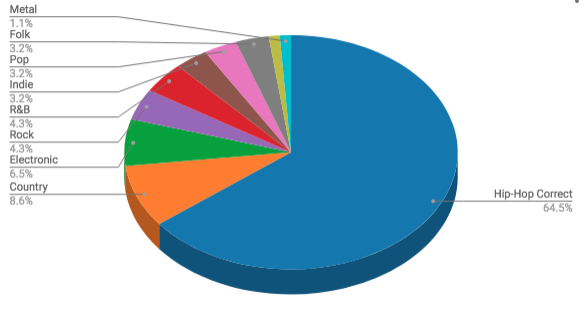
\includegraphics[width=9cm]{Figure_5}
\caption{Total 'Hip-Hop' Prediction Results}
\end{figure}

\begin{figure}[h!]
\centering
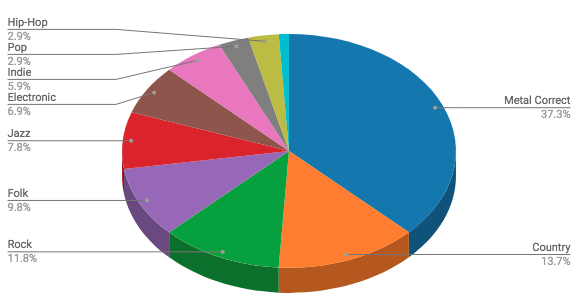
\includegraphics[width=9cm]{Figure_6}
\caption{Total 'Metal' Prediction Results}
\end{figure}

\begin{figure}[h!]
\centering
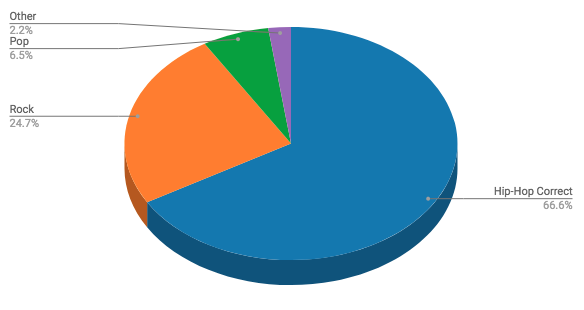
\includegraphics[width=9cm]{Figure_2}
\caption{Total 'Hip-Hop' Prediction Results}
\end{figure}

\begin{figure}[h!]
\centering
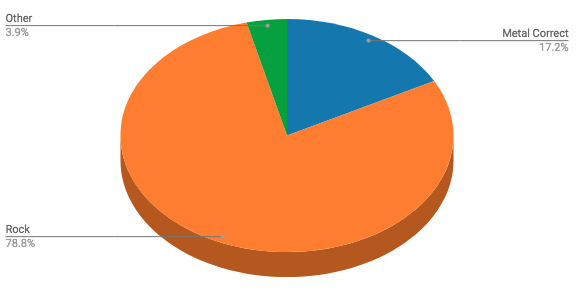
\includegraphics[width=9cm]{Figure_3}
\caption{Total 'Metal' Prediction Results}
\end{figure}

%-------------------------------------------------------------------------------------------------------------------
\newpage
\section{RNN Results}

TODO::

\begin{table}[h!]
    \label{tab:table1}
    \caption{RNN Genre Accuracies}
    \begin{tabular}{|m{0.4cm}|m{0.5cm}|m{0.4cm}|m{0.5cm}|m{0.4cm}|m{0.4cm}|m{0.45cm}|m{0.4cm}|m{0.4cm}|m{0.4cm}}
    \textbf{Jazz} & \textbf{Metal} & \textbf{Elec.} & \textbf{Country} & \textbf{H.H} & \textbf{Indie} & \textbf{Rock} & \textbf{R\&B} & \textbf{Folk} & \textbf{Pop}\\
      \hline
      \\
	41\% & 38\% & 36\%& 33\% & 30\% & 14\% & 13\% & 10\% & 0.8\% & 0\%\\

    \end{tabular}
\end{table}

%-------------------------------------------------------------------------------------------------------------------
\section{Discussion of Results}

Even though our SVM trained on the entire cleaned dataset achieved a better overall accuracy than our SVM trained on the stratified dataset, we feel that our models trained on the stratified dataset, are more generalizable than the model created on the largely Rock dataset. For example, if our testing set for our non-stratified trained SVM did not contain such a large proportion of Rock, it is likely that it would not have performed as well as it did, and if given the testing set that was used for the stratified dataset, it is likely that it would have done worse than the models trained with the stratified dataset.

Furthermore, we feel that the models trained on the stratified dataset more accurately reflect the models that were created in related literature, thus, making the features that we extracted from the lyrics comparable to the features that were extracted in related works. After comparing our results with the genre SVMs found in related works, although we achieved a lower accuracy across the ten genres, we believe the inclusion of song metadata, such as song length, beats per minute, words per minute, etc. would be beneficial in classifying the ten available genres. Overall, we believe that our SVM was successful because of the NL features that were used in training our models. Based on our prior belief about distinguishing NL features that are found in each genre, we expected the features that we chose to be a suitable subset of the features that could potentially be extracted from purely lyrical data.


%-------------------------------------------------------------------------------------------------------------------
\section{Future Work}

To ameliorate our current supervised classifier, we would like to run the model on different subsets of the natural language features in order to find the optimal set. The SVM feature set we used focused solely on semantic elements, ignoring word identity. It would be interesting to see if accuracy would improve were word identity, perhaps using a bag of words style feature encoding, included in the SVM feature space.

Additional testing could have been performed on our stratified dataset, as due to time constraints we had to limit the number of samples from each of the different genres that were used to train our models. In particular, we were only able to train and test our SVMs with a dataset of 10,000 songs, 1,000 from each genre, however the computational time required for training our models would have been infeasible with the time constraints of the course and the computational resources that we had available. In addition, further tuning of hyper-parameters could have been performed instead of just the three set slack coefficients that we experimented with.

Similar to how we examined the misclassifications that were being made between our stratified and non-stratified trained SVMs, we would have also liked to compare the misclassifications between the stratified SVM and the Recurrent Neural Network. In doing so, we would be able to examine which genres were classifiable by word identity vs. the genres that are classifiable via semantic elements.
Based on our results, we expect that the categories of genres can be classified by both word identity and semantic elements, however, we would have still liked to further analyze which specific genres benefitted from the word identity and which benefited from the semantic elements.

%-------------------------------------------------------------------------------------------------------------------
\section{Ethical Implications}

Theoretically our models are learning the platonic ideal of a song in any given genre or that is the intent. Reverse engineering them, especially the neural network which focused on the content rather than the structure of the lyrics, could potentially generate a song with severe biases. For example, a 'prototypic' Hip-Hop song might not necessarily contain racial slurs, according to our model, but this is not true in reality.

It is also must be noted that our model is biased towards the North American perception of genre - as the data was all in english and drawn from North American sources- , which is not necessarily universal.

%-------------------------------------------------------------------------------------------------------------------
\newpage
\section{Distribution of Tasks Among Team Members}

Each team member contributed to a specific area outlined below:

\begin{table}[h!]
    \label{tab:table1}
    \begin{tabular}{l|l|l|}
      \textbf{Tasks} & \textbf{Member(s)}\\

      \hline
	Data Cleaning & Anna Sollazzo, Jordan Jay\\
	NL Feature Generation & Anna Sollazzo, Jordan Jay\\
	SVM & Anna Sollazzo, Henry Hart, Jordan Jay\\
	Neural Net & Juan Carlos Gallegos, Robert Craig\\
	Report Formatting/Latex & Henry Hart\\
	Presentation Slides & All\\

    \end{tabular}
\end{table}

\begin{thebibliography}{6}

\bibitem{tsaptsinos}
A.~Tsaptsinos, \emph{Lyrics-Based Music Genre Classification Using a Hierarchical Attention Network}, \relax ICME, Stanford University, USA, 2017.

\bibitem{NLTK}
Bird, Steven, Edward Loper and Ewan Klein (2009), \emph{Natural Language Processing with Python}. \relax O'Reilly Media Inc.

\bibitem{Yang}
Z. Yang, D. Yang, C. Dyer, X. He, A. Smola, E. Hovy (2014), \emph{Hierarchical Attention Networks for Document Classification}.

\bibitem{KaggleDataset}
GyanendraMishra (2017), \emph{380,000+ Lyrics from MetroLyrics}, https://www.kaggle.com/gyani95/380000-lyrics-from-metrolyrics.

\bibitem{canicatti}
A.~Canicatti (2016), \emph{ "Song Genre Classification via Lyric Text Mining."} \relax Proceedings of the International Conference on Data Mining (DMIN). The Steering Committee of The World Congress in Computer Science, Computer Engineering and Applied Computing (WorldComp).

\bibitem{mayer} (2008) R.~Mayer, R.~Neumayer, and A.~Rauber., \emph{" Rhyme and Style Features for Musical Genre Classification by Song Lyrics"} \relax Vortrag: International Conference on Music Information Retrieval (ISMIR) Philadeliphia, USA; 14.09. 2008-18.09. 2008; in:" Proceedings of the 9th International Conference on Music Information Retrieval",(2008), S. 337-342.

\bibitem{kaggle} Kaggle~Datasets (2017), \emph{380,000+ Lyrics From MetroLyrics}, \relax https://www.kaggle.com/gyani95/380000-lyrics-from-metrolyrics

\end{thebibliography}

%-------------------------------------------------------------------------------------------------------------------

\end{document}
